%
% file : learn_git.tex
% date : jeudi 19 décembre 2019, 13:19:09 (UTC+0100)
% author : sedelpeuch
% description :
\documentclass[a4paper,10pt]{article}
\usepackage[utf8]{inputenc}
\usepackage[T1]{fontenc}
\usepackage[french]{babel}
\usepackage{graphicx}
\usepackage{float}
\usepackage{amsmath}
\usepackage{amssymb}
\usepackage{mathrsfs}
\usepackage{color}
\usepackage{fancyhdr}
\usepackage{pdfpages}
\usepackage{layout}
\usepackage{multicol}
\usepackage{setspace}
\usepackage{csvsimple}
\usepackage[table]{xcolor}
\usepackage[colorlinks=true]{hyperref}
\usepackage{tikz, tkz-tab}
\usepackage[top=2cm,bottom=2cm,left=2cm,right=2cm]{geometry}
\usepackage{amsthm}
\usepackage{listings}
\usepackage{verbatim}
\setlength{\parindent}{0.785cm}
\setlength{\parskip}{1ex plus 0.5ex minus 0.2ex}
\newcommand{\hsp}{\hspace{20pt}}
\newcommand{\HRule}{\rule{\linewidth}{0.1mm}}

\usepackage{eso-pic,graphicx}
\usepackage{xcolor}
\begin{document}
\begin{spacing}{1.5}
\graphicspath{{image/}}
  \begin{titlepage}
\begin{sffamily}
\begin{center}
\vspace*{\stretch{1}}
\textsc{\LARGE Eirbot \\ Association de robotique de l'ENSEIRB-MATMECA}\\[2cm]
\HRule \\[0.4cm]
{\huge \bfseries Présentation des projets 2020 \\[0.4cm]}

\HRule \\[2cm]

\textsc{\Large }\\[2cm]
              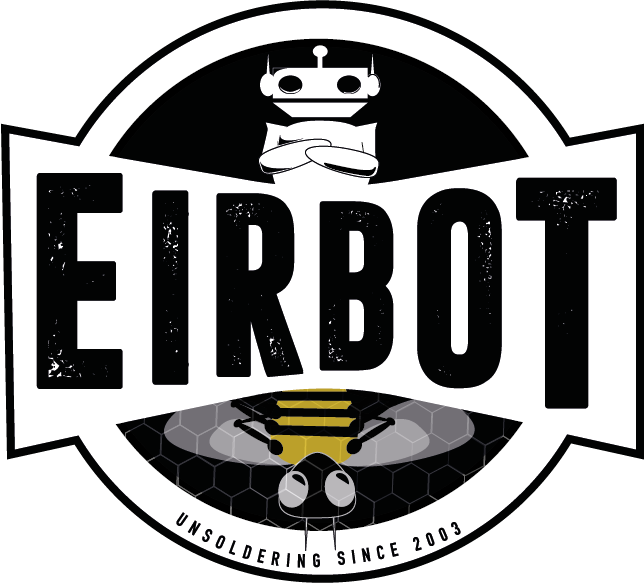
\includegraphics[scale=0.3]{LogoEirbot.png} \vfill
\vspace*{\stretch{1}}
  \end{center}
  \end{sffamily}
\end{titlepage}
\setcounter{tocdepth}{2}
\newpage
\pagestyle{fancy}
\lhead{}
\chead{\textbf{Présentation des projets 2020}}
\rhead{\thepage}
\lfoot{}
\cfoot{}
\fancyfoot[R] {
  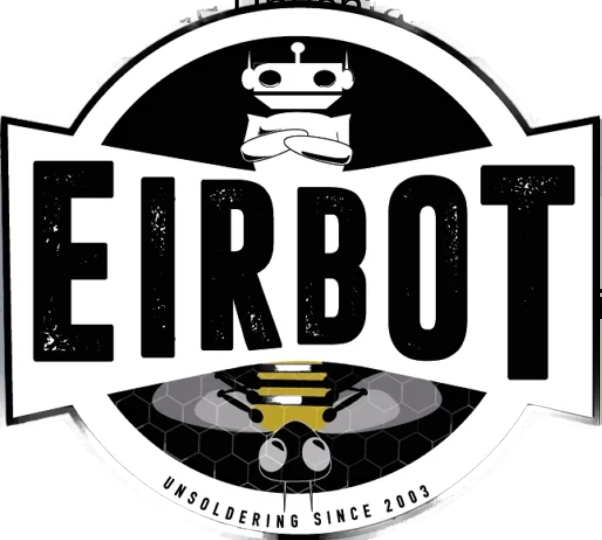
\includegraphics[scale=0.075]{65508.png} }
\section{Qui sommes nous ?}
%% Association de robotique de l'ENSEIRB-MATMECA crée en 2003, Eirbot est avant
%% tout un groupe de passionné d'électronique, d'informatique et de mécanique.
%% Chaque année, Eirbot acceuille un certain nombre d'élève ingénieur de première,
%% deuxième et troisième année. Cette année l'association contient une trentaine de membre
%% actifs. \\
%% Forte d'une équipe motivée, diversifiée, stimulée et soudée nous nous réunissons
%% autour d'un projet commun : la coupe de france de robotique. \\
%% Eirbot participe depuis sa création en tant que club (en 1997) à la coupe de
%% France de robotique
\newpage
\section{Notre Projet}
Cette année, Eirbot prend le large ! Nos robots doivent partir voguer à travers
le monde. Nous allons devoir maitriser la navigation pour arriver à bon port.
C'est après une tempête qu'il faudra reconstruire le chenal, réactiver le phare
et redresser les manches à air pour espérer gagner. Nos robots évolurons sur la
table suivante
\begin{figure}[H]
  \center
  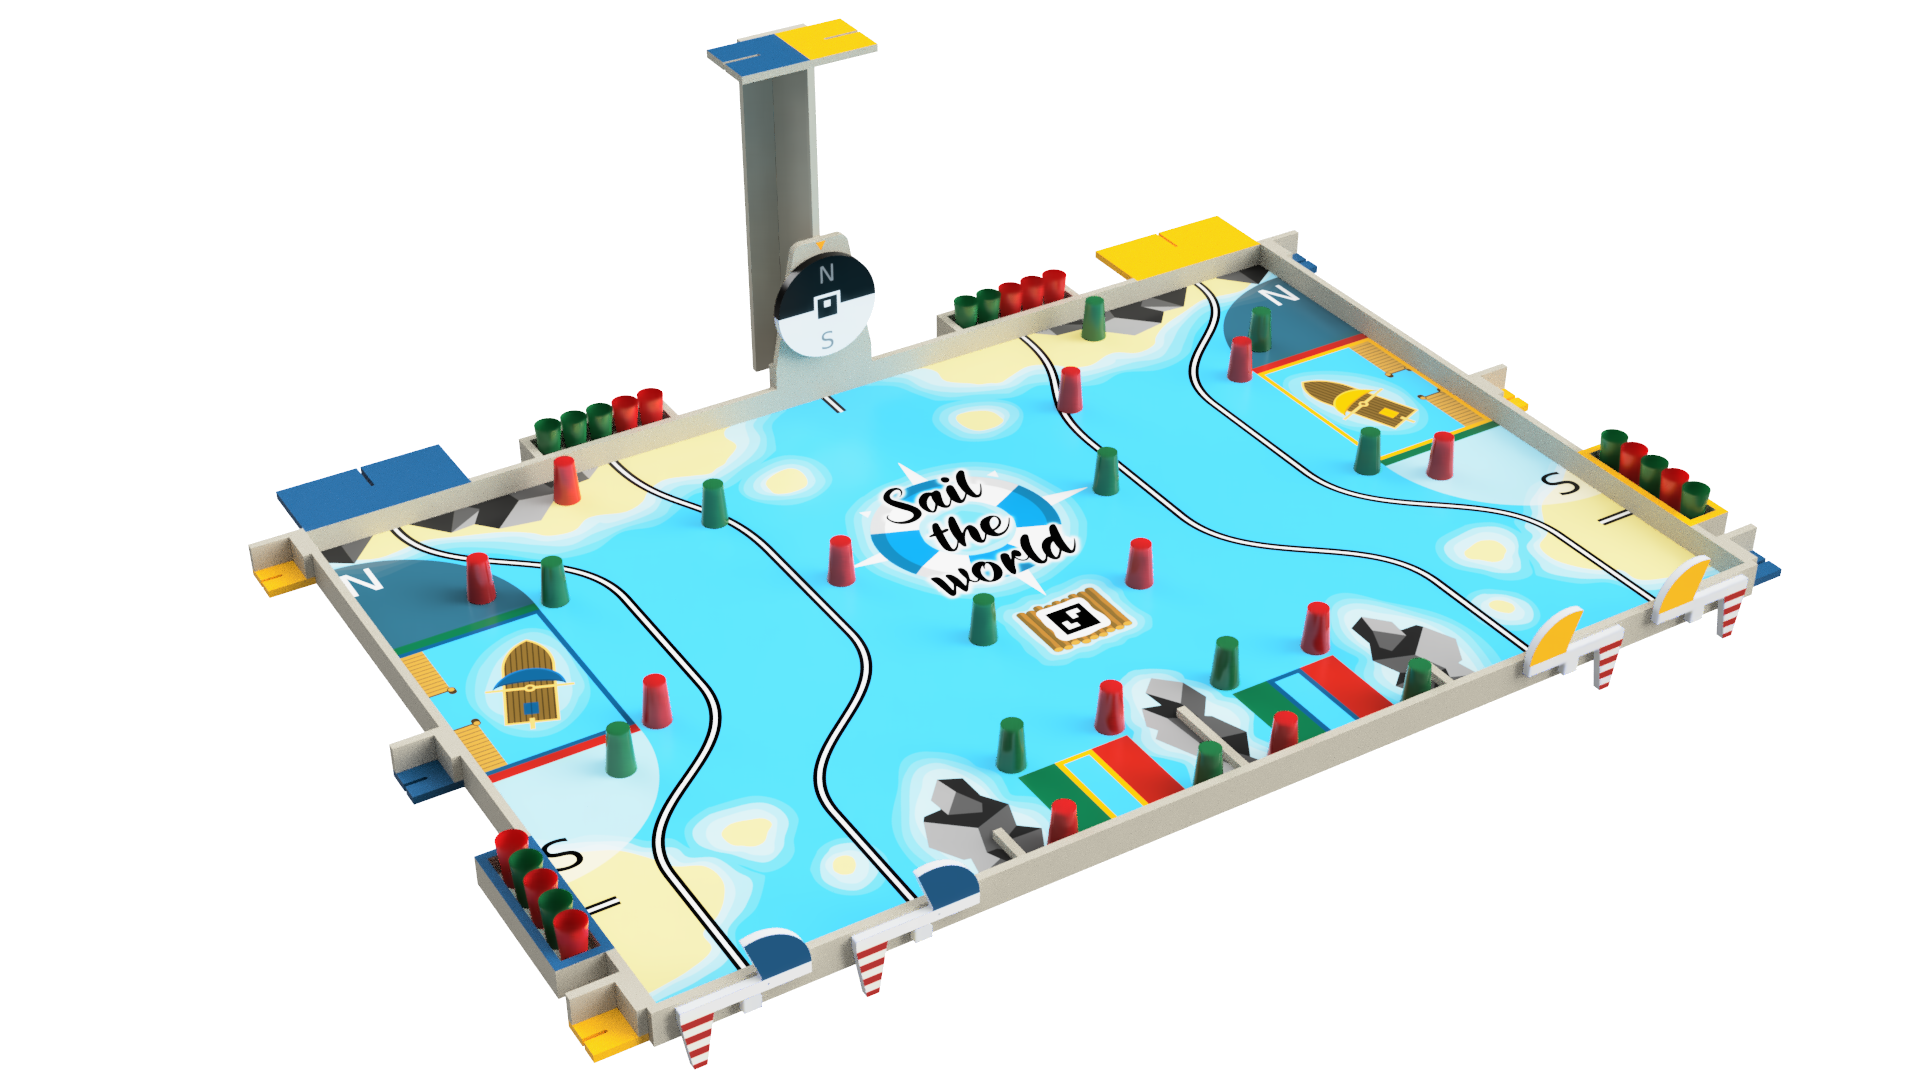
\includegraphics[scale=0.2]{table.png}
  \caption{Schéma de la table de jeu}
\end{figure}
En plus de l'environnement de jeu nous devons suivre des règles précises
disponibles sur ce \href{https://www.coupederobotique.fr/wp-content/uploads/Eurobot2020_Rules_Cup_OFFICIAL_FR.pdf}{lien}.
\subsection{Vue d'ensemble du projet et objectif de l'association}
Voyons tout d'abbord l'objectif que nous allons nous fixer pour ce projet. Nous
avons décidé en commun des différentes actions et des différentes tâches à
réaliser. Nous décidons de réaliser les actions suivantes, activer le phare,
redresser les deux manches à air, décoder la boussole et retourner à bon port.
Nous misons sur la qualité des actions et non sur la quantités de ces
dernières.

Nous avons ensuite découvert le processus de fabrication d'un robot, grâce
à l'aide des promotions supérieures nous comprenons qu'il y aura 4 grands
domaines :  la mécanique du robot (la structure, les actionneurs, le phare),
l'électronique (alimentation du robot,
contrôle des actionneurs, création du compteur de points etc), l'asservissement (direction
précise du robot) et la stratégie (recherche de chemin, choix des actions à
faire etc).
\subsection{Plans du robot}
Nous avons ensuite réalisé les plans de notre robot. Nous avons pu le rendre
concret en majeur partie grâce à la découpe laser du FabLab de l'ENSEIRB MATMECA
et à notre imprimante 3D. En addition nous utilisons des profilés pour monter la
structure et créer des étages facile à monter et démonter.
\begin{figure}[H]
  \center
  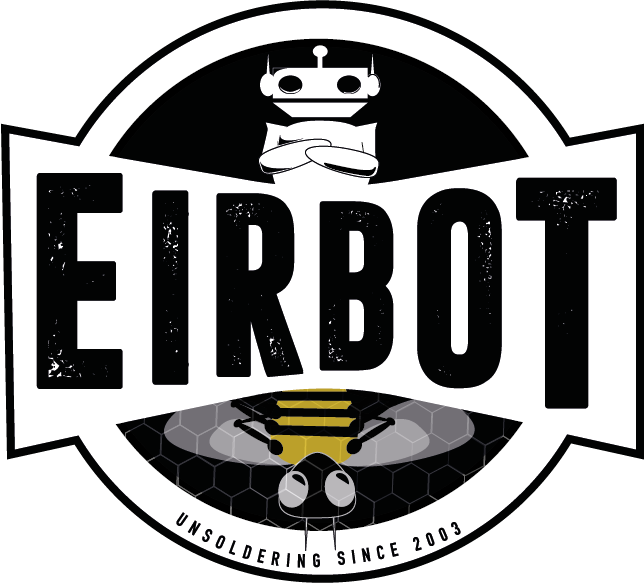
\includegraphics[scale=0.3]{LogoEirbot.png}
  \caption{Photo de l'état actuel de notre robot}
\end{figure}
Concernant notre phare, il doit se deployer et réaliser un balayage lumineux (il
doit faire moins de 30 cm avant l'activation et plus de 70 cm après). Nous optons
pour imprimer grâce à notre imprimante 3D un bras robotique, le système
d'éclairage de notre phare sera similaire à celui d'un vrai phare. Voici
l'avancement actuel de notre phare
\begin{figure}[H]
  \center
  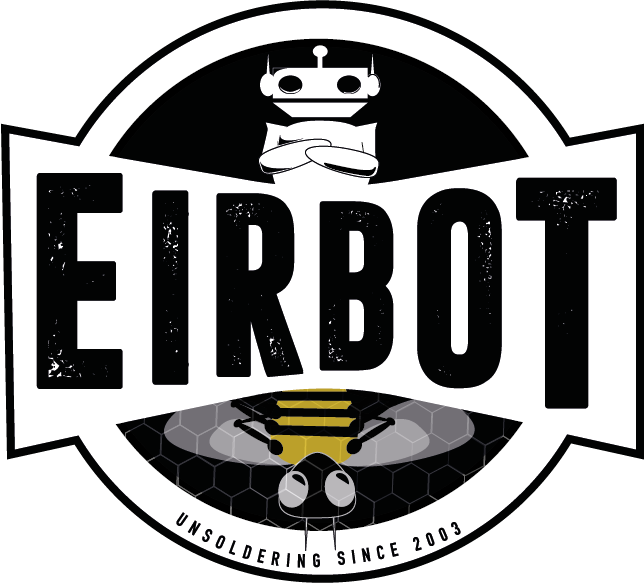
\includegraphics[scale=0.3]{LogoEirbot.png}
  \caption{Photo de l'état actuel de notre phare}
\end{figure}
\subsection{Fonctionnement général du robot}
Comme dit précédemment nous misons sur la qualité de nos actions plutôt que la
quantité. Nous divisons alors le travail informatique en deux parties. D'une
part l'Asservissement qui est implémenté sur une Nucléo-F429ZI. D'autre part, la
stratégie qui est implémentée sur une Raspberry pi 3b+. En addition nous avons du
créer un protocole de communication entre les deux cartes.\\

\subsubsection{Asservissement}
Nous pouvons commencer par décrire succinctement l'asservissement que nous avons
élaboré \\ %mettre paragraphe de clément si il existe

\subsubsection{Stratégie}
Nous pouvons maintenant décrire notre stratégie. La stratégie dépend de deux
facteurs principaux, notre capacité à naviguer sur la table et notre capacité à
détecter les adversaires et à réagir lorsque nous tombons face à l'un de.
\\ \indent Pour la navigation nous implémentons un algorithme de recherche de
chemin connu dérivé de l'algorithme de Dijikstra : l'algorithme A*. Nous
décrivons rapidement son fonctionnement dans le paragraphe suivant, une
animation expliquant le principe de ce dernier est disponible sur ce
\href{https://fr.wikipedia.org/wiki/Algorithme_A*#/media/Fichier:Astar_progress_animation.gif}{lien}.\\ \indent
Nous avons modélisé la table comme une grille chaque case faisant $1 cm \times 1
cm$. Ainsi nous avons pu renseigner la position de tous les obstacles fixes. A
partir de cela nous pouvons expliquer le fonctionnement de l'algorithme. l'A*
commence à un noeud choisi. Il applique à ce dernier un cout initial, il estime
ensuite la distance entre ce noeud et le but à atteindre. Le noeud est alors
ajouté à une liste d'attente prioritaire, appelée \textit{open list}. \\ \indent
Premièrement l'algorithme récupère le premier noeud de l'\textit{open list}. Si
elle est vide, il n'y a aucun chemin du noeud initial à celui d'arrivé,
l'algorithme est en erreur. Si le noeud est celui d'arrivé, l'algorithme va
reconstruire le chemin complet et renvoyer le résultat. Ensuite, si le noeud
n'est pas le noeud d'arrivée alors de nouveaux noeuds sont crées pour tous les
noeuds contigus admissibles . L'A* calcule ensuite son coût et le stocke avec le
noeud. Ce coût est calculé à partir de la somme du coût de son ancêtre et du
coût de l'opération pour atteindre ce nouveau noeud. En parallèle l'algorithme
conserve la liste des noeuds qui ont été vérifiés, c'est la \textit{closed
  list}. Si un noeud nouvellement produit est déjà dans cette liste avec un coût
égal ou inférieur, on ne fait rien. Après, l'évaluation de la distance du
nouveau noeud au noeud d'arrivée est ajoutée au coût pour former l'heuristique
du noeud. Ce noeud est alors ajouté à la liste d'attente prioritaire, à moins
qu'un noeud identique dans cette liste ne possède déjà une heuristique
inférieure ou égale. Une fois ces étapes effectuées pour chaque nouveau noeud
contigu, le noeud original pris de la file d'attente prioritaire est ajouté à la
liste des noeuds vérifiés. Le prochain noeud est alors retiré de la file
d'attente prioritaire et le processus recommence.

Les détails technique des notre implémentation sont disponibles sur notre
\href{https://github.com/eirbot/eirbot2020-1A/blob/master/code/rasp/src/navigation.cpp}{Github}.
A ce stade, notre algorithme est opérationnel et nous pouvons d'un point $x,y$
donné rejoindre n'importe quel point $x',y'$ en évitant les obstacles fixes.
Nous allons maintenant présenter notre stratégie concernant les obstacles
mobiles c'est à dire les adversaires.

Nous utilisons un système infrarouge (GP2) pour la détection, ces derniers sont
placés juste au dessus des gobelets disposés sur la table (les gobelets sont
considérés comme des obstacles fixes, nous ne voulons pas les détecter avec le
système infrarouge). Lorsque nous détectons un robot adverse, la stratégie prend
un branchement, récupère l'information sur la distance que nous fournit le
système infrarouge, ajoute un obstacle puis relance la navigation ce qui permet d'éviter l'obstacle.
A la fin du branchement l'obstacle est détruit. A ce stade nous pouvons avons un
système de détection nous permettant d'éviter les robots adverses en les
contournants.

Nous avons présentés nos principales stratégies, nous n'avons pas décrit tous
nos codes mais seulement les principaux. Les autres codes sont disponibles sur
notre dépot \href{https://github.com/eirbot/eirbot2020-1A}{Github}.

\subsubsection{Protocole de communication}
En choisissant de séparer sur deux cartes différentes nos codes, nous avons une
difficulté supplémentaire qui apparait. Il faut réaliser un protocole de
communication entre les deux
%ptit lu au secours

\subsection{Electronique du robot}

\newpage
\section{Nous contacter}

\newpage
\end{spacing}
\end{document}
